\chapter{NekMesh}
\label{s:utilities:nekmesh}

\newcommand{\mc}{\texttt{NekMesh}\xspace}
\newcommand{\gmsh}{\texttt{Gmsh}\xspace}

\mc is a utility bundled with \nekpp which has two purposes:
\begin{itemize}
  \item allow foreign mesh file formats to be converted into \nekpp's XML
  format;
  \item aide in the generation of high-order meshes through a series of supplied
  processing modules.
\end{itemize}

\begin{notebox}
  \mc replaces a previous utility called MeshConvert. This change is to reflect
  the fact that the program no longer only converts and manipulates meshes but
  can now also generate them from a CAD definition. This mesh generator is in
  a early beta stage of development and as such is disabled by default. For the
  time being those not using the beta mesh generator can use \mc as they would
  have used MeshConvert, none of the functionality or methodology has changed.
\end{notebox}

There is also some limited support for other output formats. We begin by running
through a basic example to show how a mesh can be converted from the widely-used
mesh-generator \gmsh to the XML file format.

\begin{notebox}
  The default since Jan 2016 is to output the .xml files in a
  compressed form where the VERTEX, EDGES, FACES, ELEMENTS and CURVED
  information is compressed into binary format which is then
  converted into base64. This is identified for each section by the attribute
  \inltt{COMPRESSED="B64Z-LittleEndian''}.  To output
  in ascii format add the module option ``:xml:uncompress'' to the .xml file,
  i.e. \\ \inltt{ \mc file.msh newfile.xml:xml:uncompress}
\end{notebox}

\section{Exporting a mesh from \gmsh}

To demonstrate how \mc works, we will define a simple channel-like 3D geometry.
First, we must define the \gmsh geometry to be used. The \gmsh definition is
given below, and is visualised in figure~\ref{fig:util:mc:gmsh-example}.

\begin{lstlisting}[style=XmlStyle]
Point(1) = {-1, 0, 0, 1.0};
Point(2) = {-0.3, 0, 0, 1.0};
Line(3) = {1, 2};
s[] = Extrude {0, 0, 7} {
  Line{3}; Layers{5}; Recombine;
};
v[] = Extrude {{0, 0, 1}, {0, 0, 0}, Pi} {
  Surface{s[1]}; Layers{10}; Recombine;
};
\end{lstlisting}

Whilst a full tutorial on \gmsh is far beyond the scope of this document, note
the use of the \texttt{Recombine} argument. This allows us to generate a
structured hexahedral mesh; remove the first \texttt{Recombine} to generate a
prismatic mesh and both occurances to generate a tetrahedral mesh. Increasing
the \texttt{Layers} numbers refines the mesh in the radial and azimuthal
direction respectively.

\section{Defining physical surfaces and volumes}

\begin{figure}
  \begin{center}
    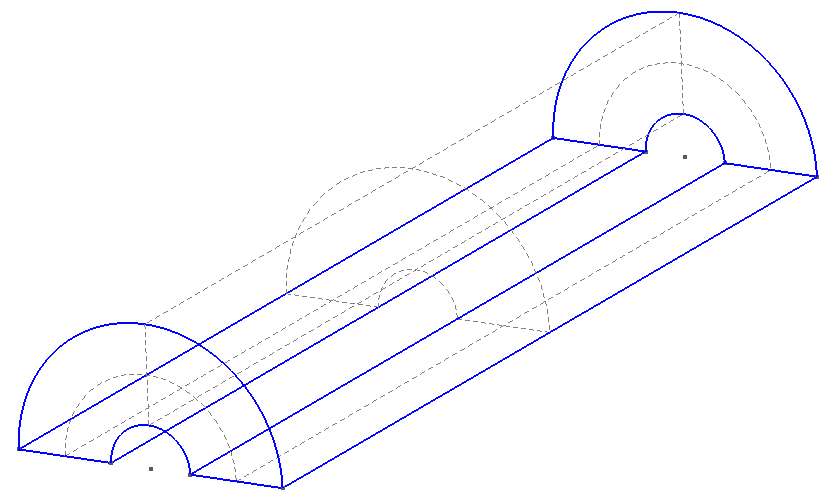
\includegraphics[width=0.4\textwidth]{img/mc-example-gmsh}
    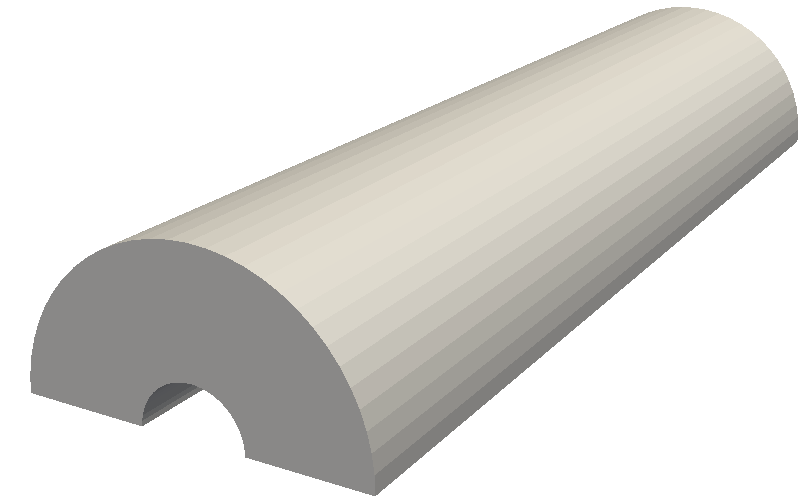
\includegraphics[width=0.4\textwidth]{img/mc-example-mesh}
  \end{center}
  \caption{Geometry definition in Gmsh (left) and resulting high-order mesh
    visualised in ParaView (right).}
  \label{fig:util:mc:gmsh-example}
\end{figure}

In order for us to use the mesh, we need to define the physical surfaces which
correspond to the inflow, outflow and walls so that we can set appropriate
boundary conditions. The numbering resulting from the extrusions in this case is
not straightforward. In the graphical interface, select \inlsh{Geometry >
  Physical Groups > Add > Surface}, and then hover over each of the surfaces
which are shown by the dashed gray lines. The numbering will be revealed in the
toolbar underneath the geometry as a ruled surface. In this case:
%
\begin{itemize}
\item \textbf{Walls:} surfaces 7, 8, 28, 29.
\item \textbf{Inflow:} surface 16.
\item \textbf{Outflow:} surface 24.
\end{itemize}
%
We also need to define the physical volumes, which can be done in a similar
fashion. For this example, there is only one volume having ID 1. Adding these
groups to the end of the \texttt{.geo} file is very straightforward:

\begin{lstlisting}[style=XmlStyle]
Physical Volume(0) = {1};
Physical Surface(1)= {7,8,28,29};
Physical Surface(2) = {16};
Physical Surface(3) = {24};
\end{lstlisting}
Either choose the option \inlsh{File->Save Mesh} or, assuming this is saved in
a file named \inlsh{test.geo}, run the command
\begin{lstlisting}[style=BashInputStyle]
gmsh -3 test.geo
\end{lstlisting}
which will produce the resulting MSH file \inlsh{test.msh}. One can generate a
high-order mesh by specifying the order on the command line, for example
\begin{lstlisting}[style=BashInputStyle]
gmsh -3 -order 6 test.geo
\end{lstlisting}
will generate a sixth-order mesh. Note that you will need to use a current
version of \gmsh in order to do this, most likely from subversion.

\section{Converting the MSH to Nektar++ format}
Assuming that you have compiled \nekpp according to the compilation
instructions, run the command
%
\begin{lstlisting}[style=BashInputStyle]
NekMesh test.msh test.xml
\end{lstlisting}
%
to generate the XML file.
%
\begin{notebox}
  This file contains only the geometry definition (and a default
  \inltt{EXPANSIONS} definition). In order to use this mesh, a
  \inltt{CONDITIONS} section must be supplied detailing the solver and
  parameters to use.
\end{notebox}
%
To validate the mesh visually, we can use a utility such as Paraview or
VisIt. To do this, run the command
%
\begin{lstlisting}[style=BashInputStyle]
XmlToVtk test.xml
\end{lstlisting}
%
which generates an unstructured VTK file \inlsh{test.vtu}.

It is possible that, when the high-order information was inserted into the mesh
by \gmsh, invalid elements are generated which self intersect. In this case, the
Jacobian of the mapping defining the curvature will have negative regions, which
will generate warnings such as:
\begin{lstlisting}[style=BashInputStyle]
Warning: Level 0 assertion violation
3D deformed Jacobian not positive (element ID = 48) (first vertex ID = 105)
\end{lstlisting}
This tells you the element ID that is invalid, and the ID of the first vertex of
the element. Whilst a resulting simulation may run, the results may not be valid
because of this problem, or excessively large amounts of time may be needed to
solve the resulting linear system.

\section{NekMesh modules}

\mc is designed to provide a pipeline approach to mesh generation. To do this,
we break up tasks into three different types. Each task is called a
\emph{module} and a chain of modules specifies the pipeline.
%
\begin{itemize}
  \item \textbf{Input} modules read meshes in a variety of formats;
  \item \textbf{Processing} modules modify meshes to aide in generation processes;
  \item \textbf{Output} modules write meshes in a variety of formats.
\end{itemize}
%
The figure below depicts how these might be coupled together to form a pipeline:
%
\begin{figure}
  \begin{center}
    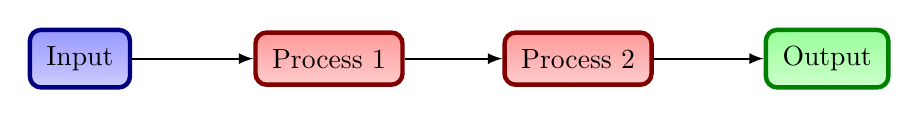
\begin{tikzpicture}[node distance=90pt]
      \tikzstyle{rect}=[line width=1.6pt,rounded corners=4pt,inner sep=6pt]
      \node[rect,top color=blue!40,bottom color=blue!20,draw=blue!50!black] (A) {Input};
      \node[rect,top color=red!40,bottom color=red!20,draw=red!50!black,right of=A] (B) {Process 1};
      \node[rect,top color=red!40,bottom color=red!20,draw=red!50!black,right of=B] (C) {Process 2};
      \node[rect,top color=green!40,bottom color=green!20,draw=green!50!black,right of=C] (D) {Output};

      \draw[-latex,thick] (A) -- (B);
      \draw[-latex,thick] (B) -- (C);
      \draw[-latex,thick] (C) -- (D);
    \end{tikzpicture}
  \end{center}
  \caption{Illustrative pipeline of the \mc process.}
  \label{fig:util:mc:pipeline}
\end{figure}
%
On the command line, we would define this as:
%
\begin{lstlisting}[style=BashInputStyle]
  NekMesh -m process1 -m process2 input.msh output.xml
\end{lstlisting}
%
Process modules can also have parameters passed to them, that can take
arguments, or not.
%
\begin{lstlisting}[style=BashInputStyle]
  NekMesh -m process1:p1=123:booleanparam input.msh output.xml
\end{lstlisting}
%
To list all available modules use the \inltt{-l} command line argument:
%
\begin{lstlisting}[style=BashInputStyle]
  Available classes:
    Input: dat:
      Reads Tecplot polyhedron ascii format converted from Star CCM (.dat).
  ...
\end{lstlisting}
%
and then to see the options for a particular module, use the \inltt{-p} command
line argument:
%
\begin{lstlisting}[style=BashInputStyle]
  Options for module detect:
          vol: Tag identifying surface to process.
\end{lstlisting}
%
\begin{notebox}
  Module names change when you use the \inltt{-p} option. Input modules should
  be preceded by \inltt{in:}, processing modules by \inltt{proc:} and output
  modules by \inltt{out:}.
\end{notebox}

\subsection{Input modules}

Input and output modules use file extension names to determine the correct
module to use. Not every module is capable of reading high-order information,
where it exists. The table below indicates support currently implemented.

\begin{center}
  \begin{tabularx}{\linewidth}{llcX}
    \toprule
    \textbf{Format} & \textbf{Extension} & \textbf{High-order} & \textbf{Notes}\\
    \midrule
    Gmsh & \texttt{msh} & \cmark & Only reads nodes, elements and physical groups (which are mapped to composites).\\
    Nektar & \texttt{rea} & \cmark & Reads elements, fluid boundary conditions. Most curve types are unsupported: high-order information must be defined in an accompanying .hsf file. \\
    Nektar++ & \texttt{xml} & \cmark & Fully supported. \\
    PLY & \texttt{ply} & \xmark & Reads only the ASCII format.. \\
    Semtex & \texttt{sem} & \cmark & Reads elements and boundary conditions. In order to read high-order information, run \inltt{meshpr session.sem > session.msh} and place in the same directory as the session file.\\
    Star-CCM+ & \texttt{dat} & \xmark & Star outputs plt file which currently needs to be coverted to ascii using Tecplot. Reads mesh only, only support for quads and triangles (2D) and hexes, prisms, tetrahedra (3D).\\
    Star-CCM+ & \texttt{ccm} & \xmark & Reads start ccm format. Reads mesh only, only support for quads and triangles (2D) and hexes, prisms, tetrahedra (3D). Requires NEKTAR\_USE\_CCM option to be activated in cmake and then requires ccmio library to be compiled by user.  \\
    VTK & \texttt{vtk} & \xmark & Experimental support. Only ASCII triangular data is supported. \\
    \bottomrule
  \end{tabularx}
\end{center}

Note that you can override the module used on the command line. For example,
\texttt{Semtex} session files rarely have extensions. So for a session called
\inltt{pipe-3d} we can convert this using the syntax
%
\begin{lstlisting}[style=BashInputStyle]
NekMesh pipe-3d:sem pipe-3d.xml
\end{lstlisting}

Typically, mesh generators allow physical surfaces and volumes to contain many
element types; for example a cube could be constructed from a mixture of hexes
and prisms. In \nekpp, a composite can only contain a single element
type. Whilst the converter will attempt to preserve the numbering of composites
from the original mesh type, sometimes a renumbering will occur when a domain
contains many element types. For example, for a domain with the tag \inltt{150}
containing quadrilaterals and triangles, the Gmsh reader will print a
notification along the lines of:

\begin{lstlisting}[style=BashInputStyle]
Multiple elements in composite detected; remapped:
- Tag 150 => 150 (Triangle), 151 (Quadrilateral)
\end{lstlisting}

The resulting file therefore has two composites of IDs \inltt{150} and
\inltt{151} respectively, containing the triangular and quadrilateral elements
of the original mesh.

\subsection{Output modules}

The following output formats are supported:

\begin{center}
  \begin{tabularx}{\linewidth}{llcX}
    \toprule
    \textbf{Format} & \textbf{Extension} & \textbf{High-order} & \textbf{Notes}\\
    \midrule
    Gmsh & \texttt{msh} & \cmark & Curvature output is highly experimental.\\
    Nektar++ & \texttt{xml} & \cmark & Most functionality supported. \\
    VTK & \texttt{vtk} & \xmark & Experimental. Only ASCII triangular data is supported. \\
    \bottomrule
  \end{tabularx}
\end{center}

Note that for both \gmsh and \texttt{VTK}, it is highly likely that you will
need to experiment with the source code in order to successfully generate
meshes since robustness is not guaranteed.

The default for \texttt{xml} is into binary data which has been
converted into base64. If you wish to see an ascii output you need to
specify the output module option \inltt{uncompress} by executing:

\begin{lstlisting}[style=BashInputStyle]
NekMesh Mesh.msh output.xml:xml:uncompress
\end{lstlisting}

In the rest of these subsections, we discuss the various processing modules
available within \mc.

\subsection{Extract surfaces from a mesh}
\label{s:utilities:nekmesh:extract}

Often one wants to visualise surfaces of a 3D mesh, or extract the values of
variables on the surface and visualise them. To support this, \mc can extract
two-dimensional surfaces which can be visualised using \inltt{FieldConvert} in
order to extract the value of a 3D field on a given surface.

As an example, we can extract composite surfaces 2 and 3-5 from a mesh using the
\inltt{extract} module:
%
\begin{lstlisting}[style=BashInputStyle]
NekMesh -m extract:surf=2,3-5 Mesh.xml output.xml
\end{lstlisting}
%
If you also wish to have the boundaries of the extracted surface detected add
the \inltt{detectbnd} option
%
\begin{lstlisting}[style=BashInputStyle]
NekMesh -m extract:surf=2,3-5:detectbnd Mesh.xml output.xml
\end{lstlisting}
which will produce new composites for the extracted boundary.

\subsection{Negative Jacobian detection}

To detect elements with negative Jacobian determinant, use the \inltt{jac}
module:
%
\begin{lstlisting}[style=BashInputStyle]
NekMesh -m jac Mesh.xml output.xml
\end{lstlisting}
%
To get a detailed list of elements which have negative Jacobians, one may use
the \inltt{list} option:
%
\begin{lstlisting}[style=BashInputStyle]
NekMesh -m jac:list Mesh.xml output.xml
\end{lstlisting}
%
and to extract the elements for the purposes of visualisation within the domain,
use the \inltt{extract} boolean parameter:
%
\begin{lstlisting}[style=BashInputStyle]
NekMesh -m jac:extract Mesh.xml MeshWithNegativeElements.xml
\end{lstlisting}

To turn off curvature associated with negative jacobians one can try to use the \inltt{removecurveifsingular} boolean parameter:
\begin{lstlisting}[style=BashInputStyle]
NekMesh -m jac:removecurveifsingular  Mesh.xml output.xml
\end{lstlisting}
This option will remove the high order curvature on prismatic faces
with singular jacobians. This does not guarantee a non-singular mesh
since it is possible for neighbouring element then to have singular
jacobians. Multiple calls to the module might help with this scenario.

\subsection{Spherigon patches}

Where high-order information is not available (e.g. when using meshes from
imaging software), various techniques can be used to apply a smoothing to the
high-order element. In \mc we use \emph{spherigons}, a kind of patch used in the
computer graphics community used for efficiently smoothing polygon surfaces.

Spherigons work through the use of surface normals, where in this sense
`surface' refers to the underlying geometry. If we have either the exact or
approximate surface normal at each given vertex, spherigon patches approximate
the edges connecting two vertices by arcs of a circle. In \mc we can either
approximate the surface normals from the linear elements which connect to each
vertex (this is done by default), or supply a file which gives the surface
normals.

To apply spherigon patches on two connected surfaces 11 and 12 use the following
command:
%
\begin{lstlisting}[style=BashInputStyle]
NekMesh -m spherigon:surf=11,12 \
    MeshWithStraighEdges.xml MeshWithSpherigons.xml
\end{lstlisting}
%
If the two surfaces "11" and "12" are not connected, or connect at a sharp edge
which is $C^0$ continuous but not $C^1$ smooth, use two separate instances of
the spherigon module.
%
\begin{lstlisting}[style=BashInputStyle]
NekMesh -m spherigon:surf=11 -m spherigon:surf=12 \
    MeshWithStraighEdges.xml MeshWithSpherigons.xml
\end{lstlisting}
%
This is to avoid the approximated surface normals being incorrect at the edge.

If you have a high-resolution mesh of the surfaces 11 and 12 in \inltt{ply}
format it can be used to improve the normal definition of the spherigons. Run:
\begin{lstlisting}[style=BashInputStyle]
NekMesh -m spherigon:surf=11,12:usenormalfile=Surf_11-12_Mesh.ply \
    MeshWithStraighEdges.xml MeshWithSpherigons.xml
\end{lstlisting}

This can be useful, for example, when meshing the Leading edge of an
airfoil. Starting from a linear mesh (left figure) the spherigon patches curve
the surface elements producing leading edge closer to the underlying geometry:

\begin{figure}[!htbp]
  \begin{center}
    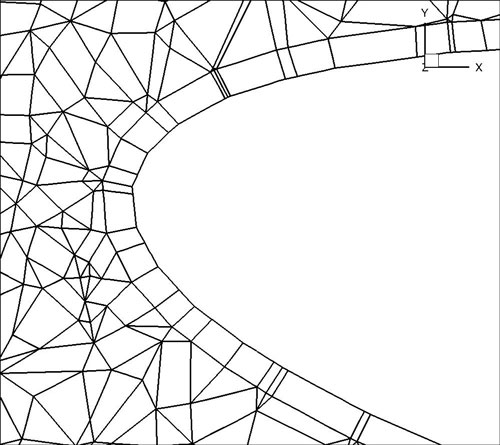
\includegraphics[width = 0.47 \textwidth]{img/noSphnoBL.jpg}
    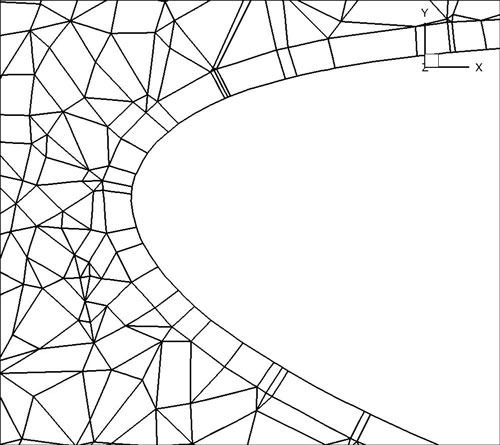
\includegraphics[width = 0.47 \textwidth]{img/SphnoBL.jpg}
    \caption{(a) Leading edge without spherigons, (b) Leading edge with
      spherigons}
  \end{center}
\end{figure}

\subsection{Periodic boundary condition alignment}

When using periodic boundary conditions, the order of the elements within the
boundary composite determines which element edges are periodic with the
corresponding boundary composite.

To counteract this issue, \mc has a periodic alignment module which attempts to
identify pairs of mutually periodic edges. Given two surfaces \inltt{surf1} and
\inltt{surf2}, which for example correspond to the physical surface IDs
specified in \gmsh, and an axis which defines the periodicity direction, the
following command attempts to reorder the composites:
%
\begin{lstlisting}[style=BashInputStyle]
NekMesh -m peralign:surf1=11:surf2=12:dir=y \
    -m peralign:surf1=13:surf2=14:dir=z Mesh.xml Mesh_aligned.xml
\end{lstlisting}
%
Here the surfaces with IDs 11 and 12 will be aligned normal to the $y$-axis and
the surfaces 13 and 14 will be aligned normal to the $z$-axis.

Note that this command cannot perform magic -- it assumes that any given edge or
face lying on the surface is periodic with another face on the opposing surface,
that there are the same number of elements on both surfaces, and the
corresponding edge or face is the same size and shape but translated along the
appropriate axis.

In 3D, where prismatic or tetrahedral elements are connected to one or both of
the surfaces, additional logic is needed to guarantee connectivity in the XML
file. In this case we append the \inltt{orient} parameter:
%
\begin{lstlisting}[style=BashInputStyle]
NekMesh -m peralign:surf1=11:surf2=12:dir=y:orient input.dat output.xml
\end{lstlisting}

\begin{notebox}
  One of the present shortcomings of \inltt{orient} is that it throws away all
  high-order information and works only on the linear element. This can be
  gotten around if you are just doing e.g. spherigon patches by running this
  \inltt{peralign} module before the \inltt{spherigon} module.
\end{notebox}

\subsection{Boundary layer splitting}

Often it is the case that one can generate a coarse boundary layer grid of a
mesh. \mc has a method for splitting prismatic and hexahedral elements into
finer elements based on the work presented in~\cite{MoHaPeSh14}
and~\cite{MoHaPeSh14b}. You must have a prismatic mesh that is $O$-type -- that
is, you can modify the boundary layer without modifying the rest of the mesh.

Given $n$ layers, and a ratio $r$ which defines the relative heights of elements
in different layers, the method works by defining a geometric progression of
points
\[
x_k = x_{k-1} + ar^k, \quad a = \frac{2(1-r)}{1 - r^{n+1}}
\]
in the standard segment $[-1,1]$. These are then projected into the coarse
elements to construct a sequence of increasingly refined elements, as depicted
in figure~\ref{fig:util:mc:split}.

\begin{figure}
  \begin{center}
    \begin{tikzpicture}
      \node[above right] at (0,0){%
        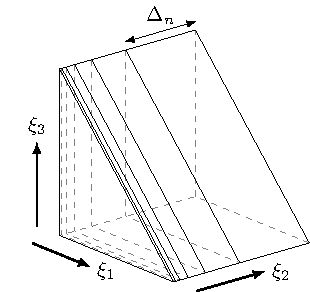
\includegraphics{img/stdprism_split}};
      \node[above right] at (6,0){%
        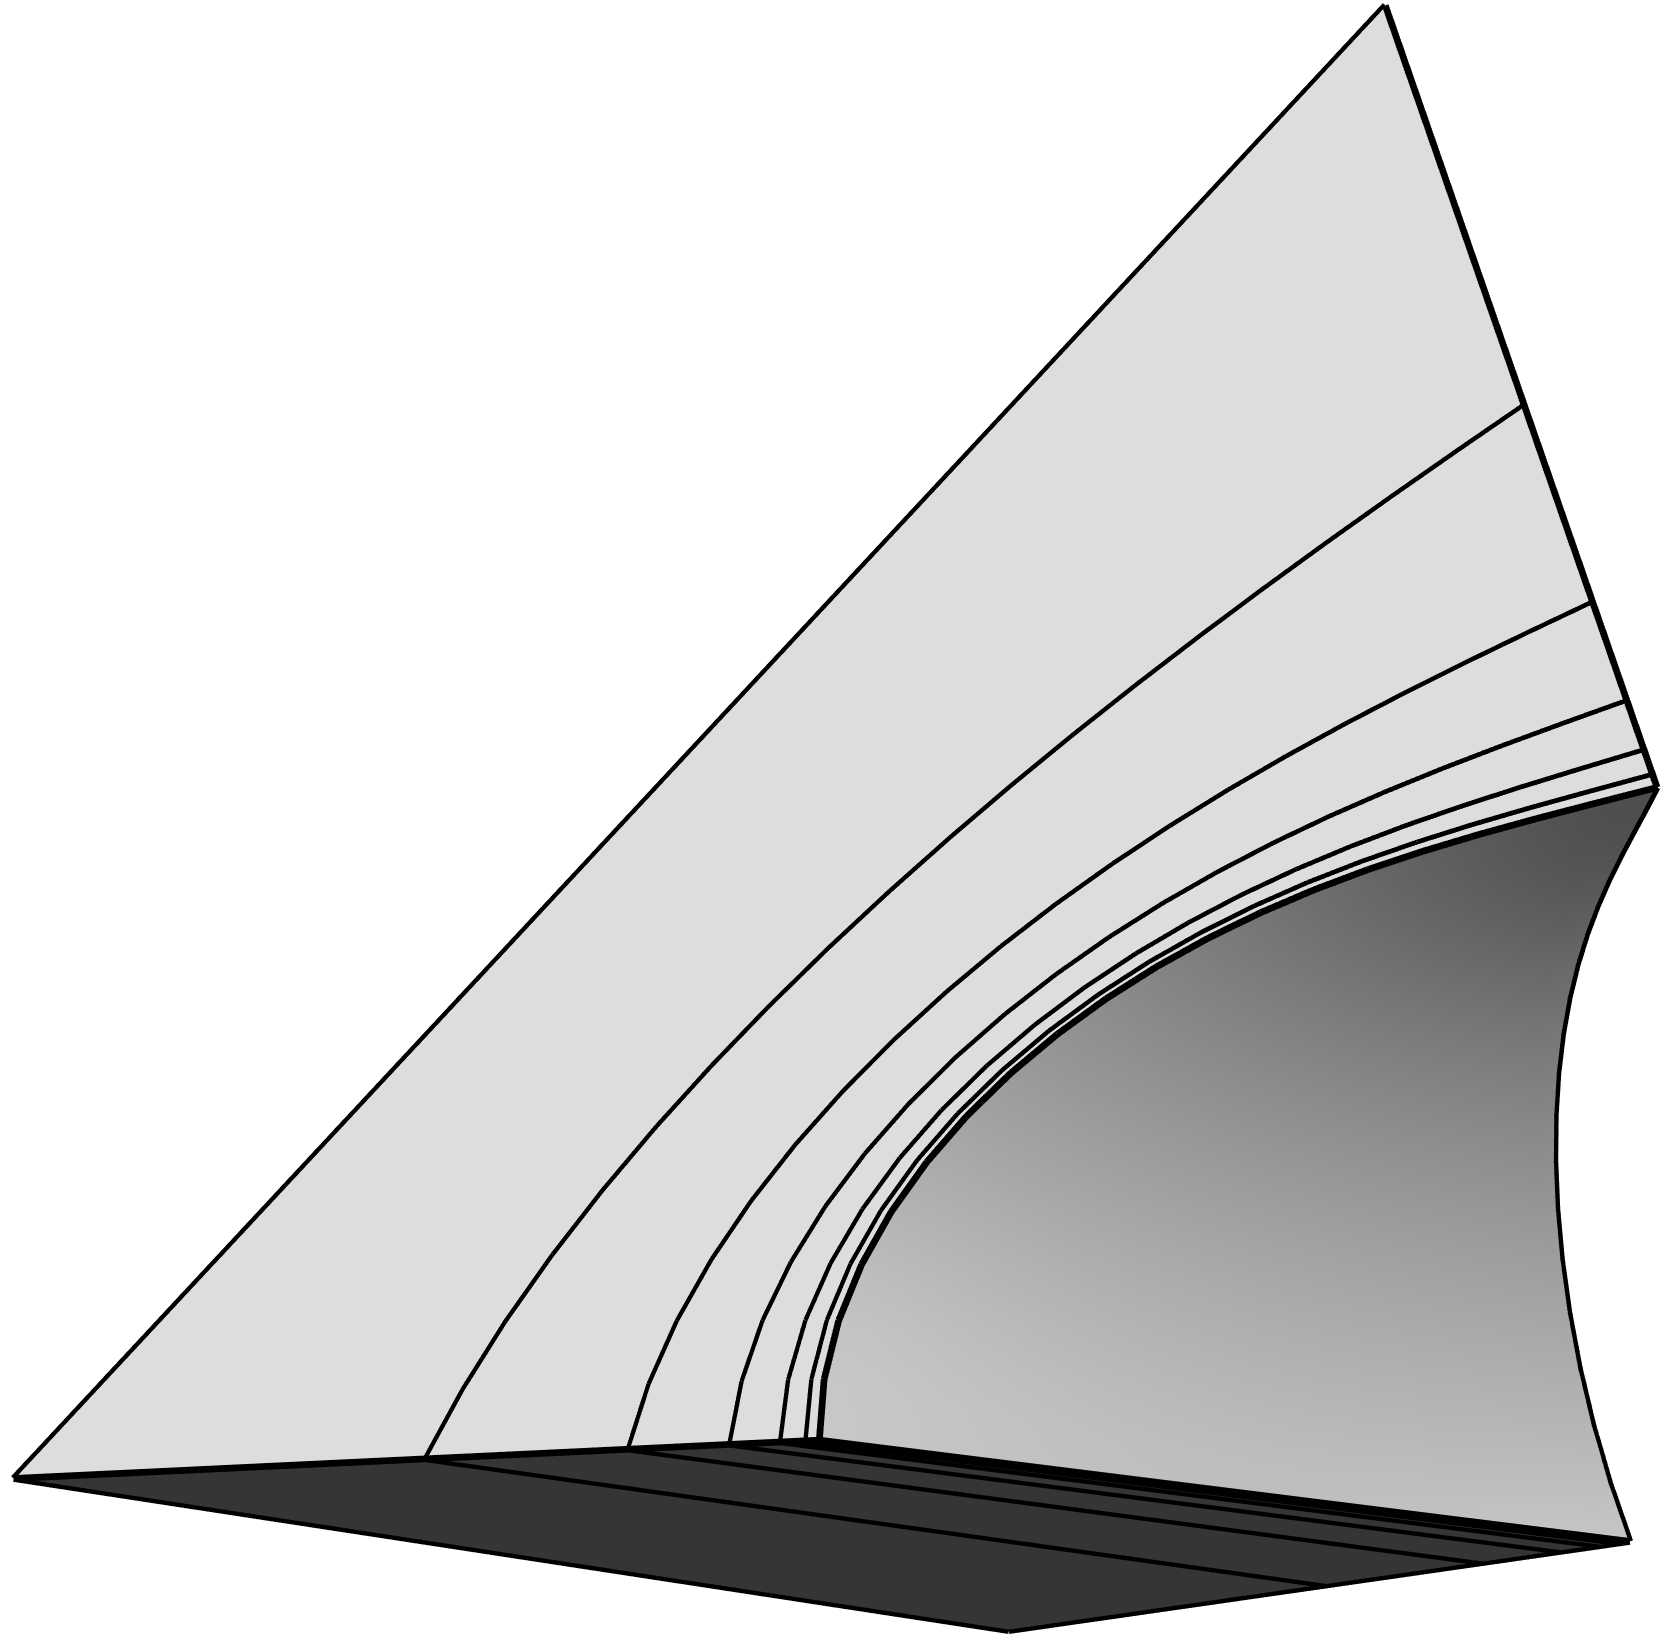
\includegraphics[width=5cm]{img/prism_split}};
      \draw[-latex,thick,bend left] (4.5,3.75) to[bend left]
      node[midway,above] {$\chi^e(\mathbf{\xi})$} (8.5,3.75);
    \end{tikzpicture}
  \end{center}
  \caption{Splitting $\Omega_{\text{st}}$ and applying the mapping $\chi^e$ to
    obtain a high-order layer of prisms from the macro-element.}
  \label{fig:util:mc:split}
\end{figure}

To split a prism boundary layer on surface 11 into 3 layers with a growth rate
of 2 and 7 integration points per element use the following command:
\begin{lstlisting}[style=BashInputStyle]
  NekMesh -m bl:surf=11:layers=3:r=2:nq=7 MeshWithOnePrismLayer.xml \
        MeshWith3PrismsLayers.xml
\end{lstlisting}
%
\begin{figure}[!htbp]
  \begin{center}
    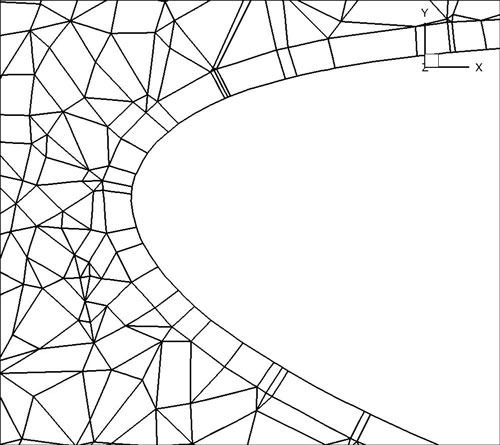
\includegraphics[width = 0.47 \textwidth]{img/SphnoBL.jpg}
    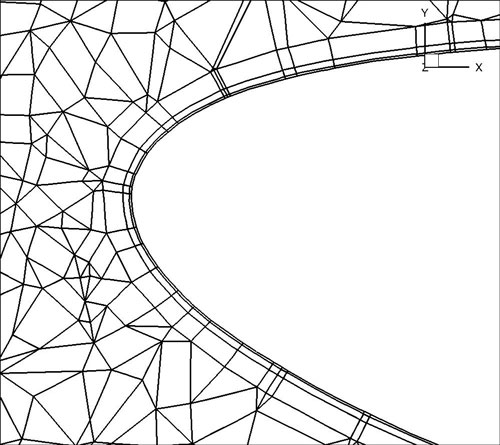
\includegraphics[width = 0.47 \textwidth]{img/SphBL.jpg}
    \caption{(a) LE with Spherigons but only one prism layer for resolving the
      boundary layer, (b) LE with Spherigons with 3 growing layers of prisms for
      better resolving the boundary layer.}
  \end{center}
\end{figure}

\begin{notebox}
  You can also use an expression in terms of coordinates $(x,y,z)$ for $r$ to
  make the ratio spatially varying; e.g. \inltt{r=sin(x)}. In this case the
  function should be sufficiently smooth to prevent the elements
  self-intersecting.
\end{notebox}

\subsection{High-order cylinder generation}

Generating accurate high-order curved geometries in \gmsh is quite challenging.
This module processes an existing linear cylindrical mesh, with axis aligned
with the $z$-coordinate axis, to generate accurate high-order curvature
information along the edges.

\begin{lstlisting}[style=BashInputStyle]
NekMesh -m cyl:surf=2:r=1.0:N=5 LinearCylinder.xml HighOrderCylinder.xml
\end{lstlisting}

The module parameters are:

\begin{itemize}
  \item \inlsh{surf}: Surface on which to apply curvature. This should be the
  outer surface of the cylinder.
  \item \inlsh{r}: Radius of the cylinder.
  \item \inlsh{N}: Number of high-order points along each element edge.
\end{itemize}

\begin{notebox}
  The module could also be used to apply curvature along the interior of a
  hollow cylinder. However, there are no checks to ensure the resulting elements
  are not self-intersecting.
\end{notebox}

\subsection{Linearisation}

The ability to remove all the high-order information in a mesh can be useful
at times.

To do this in NekMesh use the command:

\begin{lstlisting}[style=BashInputStyle]
  NekMesh -m linearise high-order-mesh.xml linear-mesh.xml
\end{lstlisting}

The output will contain only the linear mesh information, all curved information
is removed.

\subsection{Extracting interface between tetrahedra and prismatic elements}

When the mesh is three-dimensional and comprised of a prismatic boundary layer
with tetrahedra in the interior of the domain, this module extracts the
prismatic elements only, and constructs a boundary region for the interface
between the tetrahedra and prisms. This is useful in, for example, the study of
aortic flows, where the prismatic boundary layer can be extracted and refined to
study unsteady advection-diffusion problems on a more refined grid inside the
boundary layer.

To use this module you therefore use the command:

\begin{lstlisting}[style=BashInputStyle]
  NekMesh -m extracttetprisminterface input.xml output.xml
\end{lstlisting}

There are no configuration options for this module, as it is highly specific to
a certain class of meshes.

\subsection{Boundary identification}

Some mesh formats lack the ability to identify boundaries of the domain they
discretise. \mc has a rudimentary boundary identification routine for conformal
meshes, which will create a composite of edges (2D) or faces (3D) which are
connected to precisely one element. This can be done using the \inltt{detect}
module:

\begin{lstlisting}[style=BashInputStyle]
  NekMesh -m detect volume.xml volumeWithBoundaryComposite.xml
\end{lstlisting}

\subsection{Scalar function curvature}

This module imposes curvature on a surface given a scalar function
$z=f(x,y)$. For example, if on surface 1 we wish to apply a surface defined by a
Gaussian $z = \exp[-(x^2+y^2)]$ using 7 quadrature points in each direction, we
may issue the command

\begin{lstlisting}[style=BashInputStyle]
  NekMesh -m scalar:surf=1:nq=7:scalar=exp\(x*x+y*y\) mesh.xml deformed.xml
\end{lstlisting}

\begin{notebox}
  This module makes no attempt to apply the curvature to the interior of the
  domain. Elements must therefore be coarse in order to prevent
  self-intersection. If a boundary layer is required, one option is to use this
  module in combination with the splitting module described earlier.
\end{notebox}


%%%%%%%%%%%%%%%%%%%%%%%%%%%%%%%%%%%%%
%%%%%%%%%%%%%%%%%%%%%%%%%%%%%%%%%%%%%

\section{Mesh generation}

In addition to the functionality described previously, \mc is capable of
generating high-order meshes directly from a CAD definition.
By default this functionality is not activated, a user wishing to utilise the
mesh generation capability of \mc must compile \nekpp with the MESHGEN option
on. As well as compiling the relevant routines into \mc it will also download
a number of other packages which are required.

As with all tasks within \mc the new mesh generation capability exists as its
own separate module which is of type Input. Due to the vast amount of code
associated with the generation of high-order meshes and the comparatively small
nature of modules in the \mc program a new library has been created for \nekpp
called {\em NekMeshUtils}, which contains all the core routines and classes for
the \mc mesh format as well as a series of classes for the generation of meshes.
This library also contains the CAD API for \nekpp which is used to generate the
meshes.

\subsection{Methodology}

This section outlines the approach taken by \mc to generate high-order meshes.
%
To simplify the sometimes very complicated high-order mesh generation processes
in other programs, \mc executes all the stages required to produce a high-order
mesh in one single pipeline which once started requires no interaction from the
user. In broad terms these stages are:
\begin{itemize}
	\item Specification of the element sizes in the mesh,
	\item Coarse linear mesh generation of the domain,
	\item Generation of optimised high-order surface on the geometric boundary,
\end{itemize}
%
and are outlined in more detail in the following sections.

\subsubsection{CAD Interaction}

At the core of all the ideas in the \mc generator is that the final mesh is a
high quality representation of the underlying geometry. As such all of the
entities in the mesh must know where they are located with respect to the CAD
and the system to be able to query any geometric information at any point in the
domain easily and with accuracy. To handle this \mc has been interfaced with the
third-party suite of CAD libraries called OpenCascade. In its normal state
OpenCascade is a very large collection of libraries with tens of thousands of
functions which are simply not needed for our purposes, because of this its
installation is a very arduous and long process. Combine this with the fact that
there are dozens of versions and types of OpenCascade, such as OpenCascade
Community Edition, it is simply impossible for \mc to use already existing
OpenCascade installations on a given machine. To solve these issues, when
installing \nekpp with the mesh generator it will download pre-compiled binaries
for the relevant OS and link against those, any previously installed versions of
OpenCascade will not be searched for and therefore ignored.
%
To reduce the massively complex libraries in OpenCascade down to a manageable
set of functions to be used in \mc a set of interface classes have been created
which act as buffer between it and \nekpp. These CAD classes mean that
development of mesh generation routines is significantly easier and in the
future \nekpp developers will be able to utilise CAD information in all aspects
of the framework without having to learn OpenCascade. Another advantage with
this approach is that adding support for other CAD engines, as well as
OpenCascade, in the future should be relativity simple and will not require the
rewriting of any of the \mc code.

\subsubsection{Automatic specification of the mesh}

One of the key challenges of generating a high-order mesh is the creation of a
suitable coarse linear mesh. It is
quite difficult for a user to define a full set spacings over a whole domain
which will produce a good quality especially when aiming for coarseness. This
is tackled in \mc with a system for automatically defining a
set of smooth and coarse mesh spacings throughout the whole domain. This is
achieved using an octree description of the domain. The domain is recursively
subdivided into octants which each describe a small portion of the domain. The
level to which the domain subdivides is based on the curvature of the geometric
boundary. Higher curvature regions will subdivide to a finer level allowing for
increased control on the mesh specification and smoothness. The geometric
curvature is then related to a mesh sizing parameter and propagated throughout
the domain ensuring a smooth mesh. For those unfamiliar with octrees, it is
best to think of it as a non-conforming hexahedral mesh

\subsubsection{Linear Mesh Generation}

The first challenge mentioned in the previous section is addressed with the
\mc approach to linear mesh generation. Primarily because of the
difficulties in interfacing existing linear mesh generators for high-order
applications the decision was made to include a bespoke linear mesh generator
within the program. Compared with the mesh generators included in commercial
packages this linear mesh generator takes the quite unconventional and more
historic approach in building the mesh in a bottom up fashion from 0D to 3D.
Using this approach means it is possible to guarantee a level of boundary
conformity which direct to 3D approaches cannot at the desired level of
coarseness. In this approach, first mesh nodes are placed on the vertices of
the CAD model (0D), then the curves in the CAD are meshed in 1D using the
vertex nodes as boundaries, then the surfaces are meshed in their 2D parameter
plane using the curve meshes as boundaries and finally the 3D volume is meshed
using the surface mesh as the boundary to complete the linear mesh. In \mc, to
achieve greater robustness, the 2D mesh generation library Triangle is used and
the TetGen library for the 3D. Both of which are highly developed Delaunay based
mesh generators. As with all additional libraies in \nekpp these are
automatically downloaded and installed if needed.

\subsubsection{High-order Surface Generation}

Addition of the high-order nodes to and the curving of the mesh is very open
problem, no high-order mesh generator has solved this and while the methods
used in \mc are not 100\% full-proof, the system currently in place can create
good quality high-order curved meshes with a reasonable robustness. This area
will receive the greatest level of development in the future. The most critical
part of defining the high-order mesh is the addition of high-order nodes on the
geometric surface. The mesh generator must achieve the greatest level of
geometric accuracy as it can otherwise it will greatly affect the final flow
solutions. If the linear surface triangulation is taken to be fixed during this
process, the problem can be addressed in a element by element fashion. If the
high-order nodes are placed by simply using an affine mapping to the CAD surface
and back the resulting high-order triangle will inherit the same distortions as
the CAD surface. To solve this \mc uses a system node location optimisation in
the parameter plane of the CAD surface to ensure the high-order triangles have
as little distortion as possible while remaining exactly on the geometric
surface. To do this the system models the high-order edges and triangles as a
network of springs with an associated spring energy which is minimised using a
multidimensional Newton type optimisation procedure with a Gauss-Seidel matrix
solver.

\subsubsection{Mesh Correction}

Due to the fact that, for the time being, no consideration is given to the
curving of mesh interior entities, the curving the geometric surface can
produce meshes with invalid elements, especially in the case of Euler
type (Tetrahedra only) meshes. Two strategies exist within \nekpp to
correct these elements. Firstly killing the curvature, by removing the
curvature of invalid elements they become valid. However this has the
massive downside of compromising the geometric accuracy of the mesh but
is quick and effective, this can be enacted using the command:
\begin{lstlisting}[style=BashInputStyle]
    NekMesh -m linearise:invalid invalidMesh.xml validMesh.xml
\end{lstlisting}
%
The alternative to this is to use the linear elastic solver within \nekpp to
deform the mesh interior entities. Its use is very computationally expensive,
as with all PDE solvers, and is also not particularly robust. It can be used
with the set of commands outlined in the FieldConvert deform and displacement
modules and the section on the Linear Elastic Solver

\subsection{Mesh generation manual}

The mesh generation is executed with the command:
\begin{lstlisting}[style=BashInputStyle]
    NekMesh session.mcf mesh.xml
\end{lstlisting}
where session.mcf is a mesh configuration file which contains all the options
and parameters needed for mesh generation. At present this .mcf format is a
modified version conditions tag as used by the solvers. In the future this will
be updated to a more logical system. Below is a simple
example.
\begin{lstlisting}[style=XmlStyle]
<NEKTAR>
    <CONDITIONS>
        <SOLVERINFO>
            <I PROPERTY="CADFile" VALUE="CAD.STEP" />
            <I PROPERTY="MeshType" VALUE="EULER" />
        </SOLVERINFO>

        <PARAMETERS>
            <P> MinDelta = 0.02 </P>
            <P> MaxDelta = 1.0 </P>
            <P> EPS = 0.4 </P>
            <P> Order = 4 </P>
        </PARAMETERS>
    </CONDITIONS>
</NEKTAR>
\end{lstlisting}
In all cases the mesh generator needs two pieces of information and four
parameters. It firstly needs to know the CAD file with which to work. Secondly,
what type of mesh to make, the options are \inltt{EULER} and \inltt{BL}. In the
case of \inltt{EULER} the mesh will be made with only tetrahedra. For \inltt{BL}
the mesh generator will attempt to insert a single macro prism layer onto the
geometry surface. This option requires additional parameters. The automatic
mesh specification system requires three parameters to build the specification
of a smooth, curvature refined mesh. Firstly \inltt{MinDelta} which is the size
of the smallest element to be found in the final mesh. Secondly \inltt{MaxDelta}
which is the maximum size of an element in the mesh and lastly \inltt{EPS} which
is a sensitivity to curvature parameter with a range $1 \geq \varepsilon > 0$
which heuristically controls the size of the elements for a given degree of
curvature on the geometric surface. \inltt{Order} is the polynomial order of
the mesh to be generated. At present there is a maximum of 4 on this parameter
this will be fixed in the near future at which point it will only be limited
by \nekpp at 16.
%
When generating a boundary layer mesh a few additional parameters must be given.
An example is shown.
\begin{lstlisting}[style=XmlStyle]
<NEKTAR>
    <CONDITIONS>
        <SOLVERINFO>
            <I PROPERTY="CADFile" VALUE="CAD.STEP" />
            <I PROPERTY="MeshType" VALUE="BL" />
	        <I PROPERTY="BLSurfs" VALUE="7-32" />
        </SOLVERINFO>

        <PARAMETERS>
            <P> MinDelta = 0.02 </P>
            <P> MaxDelta = 1.0 </P>
            <P> EPS = 0.4 </P>
            <P> Order = 4 </P>
            <P> BLThick = 0.03 </P>
        </PARAMETERS>
    </CONDITIONS>
</NEKTAR>
\end{lstlisting}
A list of the CAD surfaces which will have a prism generated on is described by
\inltt{BLSurfs} and the thickness of the boundary to aim for is \inltt{BLThick}.
%
An important point to note is the identity of surfaces is given by their order
in the CAD file. Not necessarily in the order they were created or index in
CAD software. The output in XML format will flow a similar logic in composite
numbering. Composite 0 will be the tetrahedral volume, 1 the prisms. Surface
composites will be numbered 1xx where xx is the surface number in CAD. If
the geometry has more than 100 surfaces, the numbering 1xxx will be used.
Because \nekpp meshes cannot have more that one element type in a composite,
boundary composites which make up symmetry planes, which have quad elements,
will be numbered such that 1xx is the triangular elements and 2xx are the quads.
%
The mesh generator has been created with a range of error messages to aid in
debugging. If you encounter an error and the mesh generator fails, run \mc with
the verbose \inltt{-v} flag and send the stdout with the .mcf and .step files
to \inltt{m.turner14@imperial.ac.uk}. Without the feedback this functionality
cannot improve.


%%% Local Variables:
%%% mode: latex
%%% TeX-master: "../user-guide"
%%% End:
